\begin{subfigure}{16em}
	\centering
	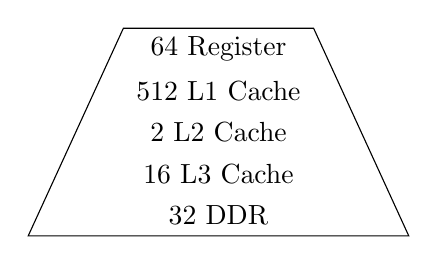
\begin{tikzpicture}[x=2.75em,y=1.5em]
		\draw (1.25, -0.5) -- ++(-2.5, 0)
			-- (-2.5, -5.5) -- ++(5, 0)
			-- cycle;
		\node at (0, -1) {$\SI{64}{\byte}$ Register};
		\node at (0, -2) {$\SI{512}{\kibi\byte}$ L1 Cache};
		\node at (0, -3) {$\SI{2}{\mebi\byte}$ L2 Cache};
		\node at (0, -4) {$\SI{16}{\mebi\byte}$ L3 Cache};
		\node at (0, -5) {$\SI{32}{\giga\byte}$ DDR};
	\end{tikzpicture}
	\caption{CPU Memory Heirarchy}
\end{subfigure}
\begin{subfigure}{16em}
	\centering
	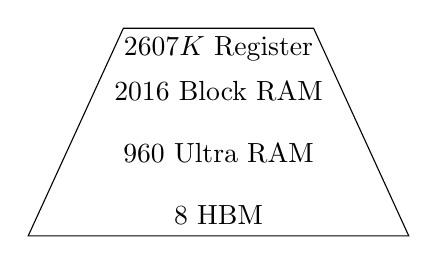
\begin{tikzpicture}[x=2.75em,y=1.5em]
		\draw (1.25, -0.5) -- ++(-2.5, 0)
			-- (-2.5, -5.5) -- ++(5, 0)
			-- cycle;
		\node at (0, -1) {$\SI{2607}{K}$ Register};
		\node at (0, -2) {$\num{2016}$ Block RAM};
		\node at (0, -3.5) {$\num{960}$ Ultra RAM};
		\node at (0, -5) {$\SI{8}{\giga\byte}$ HBM};
	\end{tikzpicture}
	\caption{FPGA Memory Heirarchy}
\end{subfigure}


% Type     | Count | Size   |
% ---------+-------+--------+
% Register | 2607K |        |
% BRAM     | 2016  | 36K    |
% URAM     |  960  | 288 Kb |
%
% Source DS963, UG440, AM007
